\documentclass[14pt, a4paper, oneside]{extarticle}
\usepackage[T2A]{fontenc}
\usepackage[utf8]{inputenc}
\usepackage[russian]{babel}
\usepackage{hyperref}
\usepackage{xcolor}
\usepackage{geometry}
\geometry{top=1cm, bottom=0.5cm, left=1cm, right=1cm}
\usepackage{graphicx}
\usepackage{float}
\usepackage{wrapfig}
\usepackage{fontawesome5}
\usepackage{ragged2e}
\usepackage{microtype}

\hypersetup{
    colorlinks=true,
    allcolors=blue,
    pdfborderstyle={/S/U/W 0},
    allbordercolors=blue
}

\begin{document}

% Фото

%\begin{wrapfigure}{l}{0.18\textwidth}
%	\vspace{\intextsep}
%    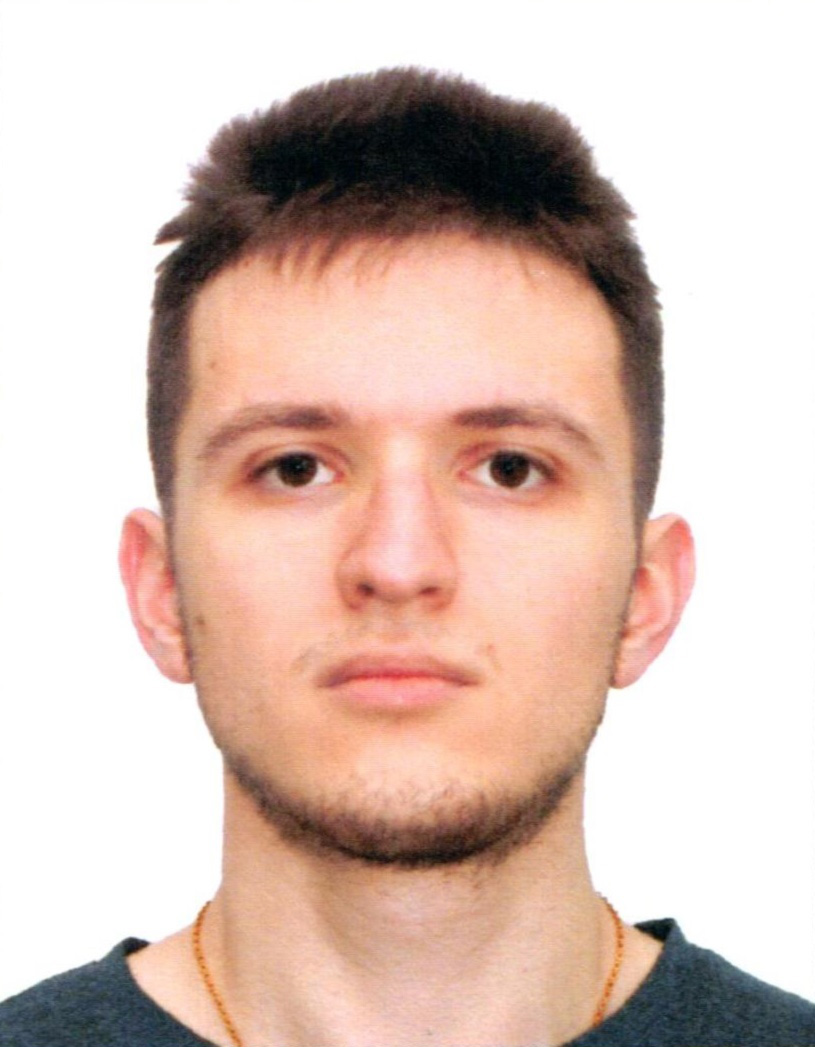
\includegraphics[width=0.18\textwidth]{personal_photo.jpg}
%\end{wrapfigure}

% Заголовок

\begin{center}
    \textbf{\LARGE Куценко Максим Дмитриевич}
    
    \textit{\Large Аналитик данных}
\end{center}

\begin{center}
	\vspace{-0.5\intextsep}
	\small
    \faPhone* \space +7 (985) 647-53-50 | \faEnvelope \space maximkuts23@gmail.com | \faGithub \space github.com/Crazy5202 | \faTelegram \space @Crazy523
\end{center}

% Подзаголовок Практический опыт

\begin{flushleft}
	\vspace{-\intextsep}
	\large Практический опыт
\end{flushleft}

\vspace{-0.8\intextsep}
\hrule

%% eComm

\begin{flushleft}
	\vspace{-0.8\intextsep}
	\quad
	\href{https://github.com/Crazy5202/eComm}{\textbf{Бэкенд интернет-магазина (учебный проект)}}
	\hfill
	Москва
\end{flushleft}

\begin{flushleft}
	\vspace{-1\intextsep}
	\quad
	\textit{Московский авиационный институт}
	\hfill
	\textit{\small Фев. 2025 - Июнь 2025}
\end{flushleft}

%%% Список eComm

\begin{itemize}
	\vspace{-2\intextsep}
	\item \href{https://github.com/Crazy5202/job_application_form/tree/main/portfolio/eComm_C4.pdf}{Микросервисная архитектура (C4)}: 4 контейнера PostgreSQL с паттерном Database per service, контейнер Elasticsearch, 4 контейнера инструментов наблюдаемости (Promtail, Prometheus, Loki, Grafana) 
	\vspace{-0.8\intextsep}
	\item Проектирование схемы БД и миграций (SQLAlchemy, Alembic)
	\vspace{-0.8\intextsep}
	\item Построение полнотекстового поиска продуктов в Elasticsearch с ETL
	
	\vspace{-0.5\intextsep} 
	изменений из основной БД PostgreSQL через CDC Debezium и Kafka
	\vspace{-0.8\intextsep}
	\item Визуальный анализ информации о метриках и логах через \href{https://github.com/Crazy5202/job_application_form/tree/main/portfolio/eComm_Grafana.pdf}{дашборд в Grafana} (Request Latency, Request Rate, Error Rate)
	\vspace{-0.8\intextsep}
    \item Руководство командой (4 человека), ведение 

    \vspace{-0.5\intextsep}
    бэклога и проектной документации (ТЗ)
    \vspace{-0.8\intextsep}
    \item Презентация результатов
\end{itemize}

%% Кинотеатр

\begin{flushleft}
	\vspace{-\intextsep}
	\quad
	\href{https://github.com/Crazy5202/Python_project}{\textbf{Онлайн-кинотеатр (учебный проект)}}
	\hfill
	Москва
\end{flushleft}

\begin{flushleft}
	\vspace{-1\intextsep}
	\quad
	\textit{Московский авиационный институт}
	\hfill
	\textit{\small Сент. 2024 - Дек. 2024}
\end{flushleft}

%%% Список Кинотеатр

\begin{itemize}
	\vspace{-2\intextsep}
	\item Организация ETL по сбору HTML-страниц фильмов из IMDB через HTTP-запросы,
    парсингу информации из них, выгрузке в БД PostgreSQL и S3-хранилище
	\vspace{-2\intextsep}
    \item Руководство командой (4 человека), ведение 

    \vspace{-0.5\intextsep}
    бэклога и проектной документации (ТЗ)
    \vspace{-0.8\intextsep}
    \item Презентация результатов
\end{itemize}

%% ЭДО

\begin{flushleft}
	\vspace{-0.8\intextsep}
	\quad
	\href{https://github.com/Crazy5202/CM_2024}{\textbf{\smallСервис распознавания подписей и печатей в документах (учебный проект)}}
	\hfill
	Москва
\end{flushleft}

\begin{flushleft}
	\vspace{-1\intextsep}
	\quad
	\textit{Московский авиационный институт, МТС}
	\hfill
	\textit{\small Фев. 2024 - Июнь 2024}
\end{flushleft}

%%% Список ЭДО

\begin{itemize}
	\vspace{-2\intextsep}
    \item Сбор и формализация бизнес-требований от \href{https://vk.ru/kearkhipov}{партнёра проекта}
	\vspace{-0.8\intextsep}
    \item Руководство командой (9 человек), ведение 
    
    \vspace{-0.5\intextsep}
    бэклога и проектной документации (ТЗ)
    \vspace{-0.8\intextsep}
    \item Презентация результатов на форуме электронного документооборота
    
    \vspace{-0.5\intextsep}
    с положительными оценками; проект рекомендован к внедрению на основе
    
    \vspace{-0.5\intextsep}
 	\href{https://github.com/Crazy5202/job_application_form/tree/main/portfolio/EDMS/%D0%9E%D1%82%D0%B7%D1%8B%D0%B2_%D0%B2%D0%BD%D0%B5%D0%B4%D1%80%D0%B5%D0%BD%D0%B8%D0%B5.pdf}{отзыва партнёра проекта} и занял \href{https://github.com/Crazy5202/job_application_form/tree/main/portfolio/EDMS/%D0%9F%D0%BE%D0%B1%D0%B5%D0%B4%D0%B8%D1%82%D0%B5%D0%BB%D1%8C_%D0%A6%D0%9A.pdf}{1 место в конкурсе на потоке}
\end{itemize}

% Новая страница

\pagebreak

% Подзаголовок Конкурсы и достижения

\begin{flushleft}
	\vspace{-\intextsep}
	\large Конкурсы и достижения
\end{flushleft}

\vspace{-0.8\intextsep}
\hrule

%% K2

\begin{flushleft}
	\vspace{-0.8\intextsep}
	\quad
	\textbf{AI Boostcamp}
	\hfill
	Москва
\end{flushleft}

\begin{flushleft}
	\vspace{-1\intextsep}
	\quad
	\textit{К2 Нейротех}
	\hfill
	\textit{\small Нояб. 2025 - Дек. 2025}
\end{flushleft}

%%% Список K2

\begin{itemize}
	\vspace{-2\intextsep}
	\item Построение RAG-системы с n8n
\end{itemize}

%% Студфест

\begin{flushleft}
	\vspace{-0.8\intextsep}
	\quad
	\textbf{Студфест 2025}
	\hfill
	Москва
\end{flushleft}

\begin{flushleft}
	\vspace{-1\intextsep}
	\quad
	\hfill
	\textit{\small Январь 2025}
\end{flushleft}

%%% Список Студфест

\begin{itemize}
	\vspace{-2\intextsep}
	\item Написание \href{https://github.com/Crazy5202/job_application_form/tree/main/portfolio/OnlyGames%5B%D0%A2ex_%D0%97%D0%B0%D0%B4%D0%B0%D0%BD%D0%B8%D0%B5%5D.pdf}{технического задания} для сайта по видеоигровой тематике
\end{itemize}

% Подзаголовок Образование

\begin{flushleft}
	\vspace{-\intextsep}
	\large Образование
\end{flushleft}

\vspace{-0.8\intextsep}
\hrule

%% Магистратура

\begin{flushleft}
	\vspace{-0.8\intextsep}
	\quad
	\textbf{Московский авиационный институт}
	\hfill
	Москва
\end{flushleft}

\begin{flushleft}
	\vspace{-\intextsep}
	\quad
	\textit{\footnotesize Магистр, %фундаментальная информатика и информационные технологии} 
	искусственный интеллект и суперкомпьютерное моделирование}
	\hfill
	\textit{\small Авг. 2026 - н.в.}
\end{flushleft}

%% ДПП по системной аналитике

\begin{flushleft}
	\vspace{-0.8\intextsep}
	\quad
	\textbf{Московский авиационный институт, Т1}
	\hfill
	Москва
\end{flushleft}

\begin{flushleft}
	\vspace{-\intextsep}
	\quad
	\href{https://github.com/Crazy5202/job_application_form/tree/main/portfolio/T1/%D0%A21_%D1%81%D0%B5%D1%80%D1%82%D0%B8%D1%84%D0%B8%D0%BA%D0%B0%D1%82.pdf}{\textit{ДПП, системный аналитик}}
	\hfill
	\textit{\small Фев. 2025 - Июнь 2025}
\end{flushleft}

%% Бакалавриат

\begin{flushleft}
	\vspace{-0.8\intextsep}
	\quad
	\textbf{Московский авиационный институт}
	\hfill
	Москва
\end{flushleft}

\begin{flushleft}
	\vspace{-\intextsep}
	\quad
	\textit{Бакалавр, прикладная математика и информатика}
	\hfill
	\textit{\small Авг. 2022 - Авг. 2026}
\end{flushleft}

% Подзаголовок Навыки

\begin{flushleft}
	\vspace{-\intextsep}
	\large Навыки
\end{flushleft}

\vspace{-0.8\intextsep}
\hrule

%% Навыки

\vspace{0.5\intextsep}

\textbf{БД и хранилища:} PostgreSQL, MongoDB, Redis, Elasticsearch, ClickHouse, S3

\textbf{Языки программирования:} SQL, Python (Flask, FastAPI, SQLAlchemy, Alembic, PySpark, asyncio, pytest)

\textbf{Трекинг задач и документация:} Jira, Trello, Confluence, Figma, MS Office

\textbf{Наблюдаемость:} Grafana, Prometheus, Loki, Promtail, Logstash, Kibana

\textbf{Инфраструктура и интеграции:} Linux, Git, Docker, Traefik, Debezium, n8n, сетевые технологии (L2/L3)

\textbf{Очереди сообщений:} Kafka, RabbitMQ

\textbf{Моделирование архитектуры и процессов:} C4, UML, BPMN, DFD, ERD, IDEF0

\textbf{Проектирование API, протоколы:} HTTP/HTTPS, REST, Swagger, JSON, XML

\textbf{Методологии:} Scrum, Kanban 

\textbf{Иностранные языки:} Английский C1

% Подзаголовок О себе

\begin{flushleft}
	\vspace{-\intextsep}
	\large О себе
\end{flushleft}

\vspace{-0.8\intextsep}
\hrule

%% О себе
\begin{sloppypar}
	\vspace{0.5\intextsep}
	\quad
	Начинающий аналитик с опытом проектирования и построения БД в микросервисной архитектуре, ETL данных, взаимодействия с командой разработки (от 4 до 9 человек), написания ТЗ. Обладаю значительным опытом использования Python для работы с СУБД и хранилищами данных. 
\end{sloppypar}

\end{document}